\section{Ejercicio 7: Dise\~no de contadores sincr\'onicos y asincr\'onicos de 3 bits}

\subsection{Contador Asincr\'onico}
En esta secci\'on se propone el dise\~no de un contador asincr\'onico de 3 bits ascendente empleando \'unicamente Flip Flops D, puesto que es el \'unico tipo de Flip Flop del cual se dispone.
Para el an\'alisis posterior se considera un contador asincr\'onico, esto \'ultimo hace referencia a que los procesos de cambios dentro del mismo no est\'an sincronizados por alg\'un evento com\'un,
sino que hay una propagaci\'on del mismo.

\subsubsection{Dise\~no del circuito}
Cada uno de los Flip Flop's corresponder\'a a un bit del contador, y para ser asincr\'onico, cada uno tiene como se\~nal de clock el complemento del bit inferior en peso, salvo el bit menos significativo cuyo clock
corresponde a una se\~nal cuadrada efectivamente. De esta forma, cada vez que se produce un cambio de estado alto a estado bajo en un bit del contador, el siguiente en peso invertir\'a su estado.
Se agrega adem\'as la posibilidad de reiniciar el contador empleando la entrada asincr\'onica de reset. Se puede observar el circuito l\'ogico resultante en la Fig. \ref{fig:esquematico_asincronico}.

En la pr\'actica se dispone de los circuitos integrados 74LS74, el cual contiene dos flip flops D independientes y necesita tener una tensi\'on de alimentaci\'on de $5V$.
Se conectan sus entradas de preset a $5V$, y luego las entradas asincr\'onicas de reset con un pull-up de $R = 100k\Omega$ a $5V$ para ofrecer al usuario la posibilidad de reiniciar el contador.

\begin{figure}[H]
    \centering
        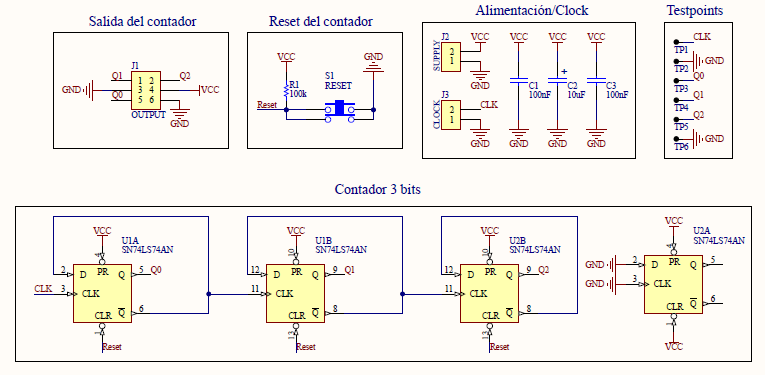
\includegraphics[scale=0.7]{../EJ7/Recursos/esquematico_asincronico.PNG}
    \caption{Esquem\'atico del PCB en Altium Designer}
    \label{fig:esquematico_asincronico}
\end{figure}

\begin{figure}[H]
    \centering
    \begin{tabular}{c c}
        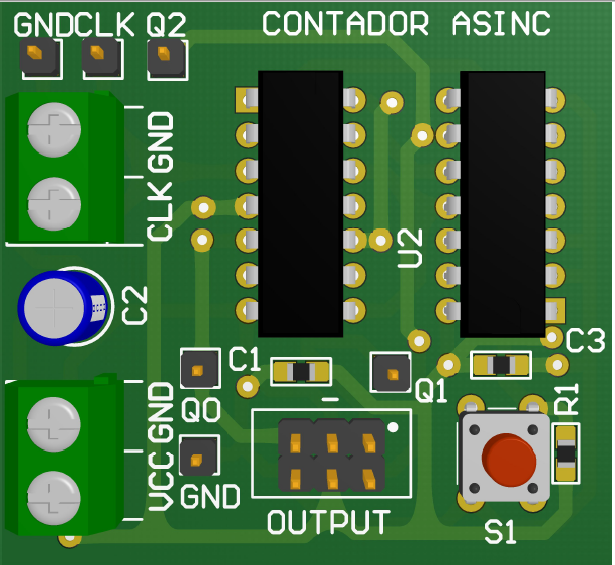
\includegraphics[scale=0.4]{../EJ7/Recursos/3d_top_asincronico.PNG} &
        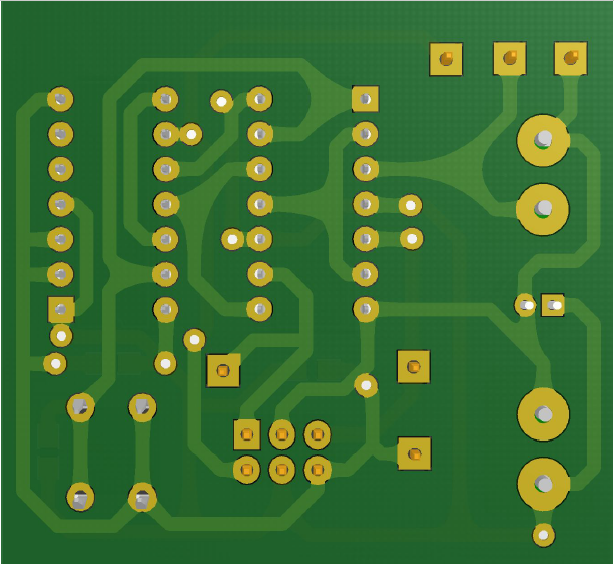
\includegraphics[scale=0.4]{../EJ7/Recursos/3d_bottom_asincronico.PNG} 
    \end{tabular}
    \caption{Dise\~no 3D del PCB}
    \label{fig:3d_asincronico}
\end{figure}

\subsection{Contador Sincr\'onico}
En esta secci\'on se propone el dise\~no de un contador sincr\'onico de 3 bits ascendente empleando \'unicamente Flip Flops D, por la misma raz\'on que para el caso asincr\'onico.
En un contador sincr\'onico, a diferencia del asincr\'onico, los proceso de cambio que ocurren en el mismo se dan sincronizados con respecto a un evento com\'un para lo cual es utilizada una se\~nal
de clock, cuyos flancos ascendentes producir\'an los cambios del contador de forma lo m\'as simult\'anea posible, ya que el evento llega de igual forma a todos y no hay una propagaci\'on como en el caso asincr\'onico.

\subsubsection{Dise\~no del circuito}
Para el circuito l\'ogico del contador se propone utilizar los flip flops como dispositivos que almacenen el estado de cada bit del contador,
luego utilizando l\'ogica externa se define c\'omo debe cambiar el estado ante un evento de sincronismo. Para ello se ilustra en la Tabla. \ref{table:tabla_verdad_contador}
la tabla de verdad del mismo. Entonces se pueden obtener las siguientes expresiones l\'ogicas:

\begin{equation}
    Q^{*}_0 = \neg Q_0 
\end{equation}

\begin{equation}
    Q^{*}_1 = Q_1 \oplus Q_0 
\end{equation}

\begin{equation}
    Q^{*}_2 = Q_2 \oplus (Q_1 \cdot Q_0) 
\end{equation}

\begin{table}[H]
    \centering
    \begin{tabular}{c c c | c c c}
        $Q_2$ & $Q_1$ & $Q_0$ & $Q^{*}_2$ & $Q^{*}_1$ & $Q^{*}_0$ \\ 
        \hline \\
        $0$ & $0$ & $0$ & $0$ & $0$ & $1$ \\
        $0$ & $0$ & $1$ & $0$ & $1$ & $0$ \\
        $0$ & $1$ & $0$ & $0$ & $1$ & $1$ \\
        $0$ & $1$ & $1$ & $1$ & $0$ & $0$ \\
        $1$ & $0$ & $0$ & $1$ & $0$ & $1$ \\
        $1$ & $0$ & $1$ & $1$ & $1$ & $0$ \\
        $1$ & $1$ & $0$ & $1$ & $1$ & $1$ \\
        $1$ & $1$ & $1$ & $0$ & $0$ & $0$ \\
    \end{tabular}
    \caption{Tabla de verdad estados actuales y futuros del contador}
    \label{table:tabla_verdad_contador}
\end{table}

Finalmente, se puede observar la implementaci\'on de estas expresiones en el circuito l\'ogico de la Fig. \ref{fig:esquematico_sincronico}.

\begin{figure}[H]
    \centering
        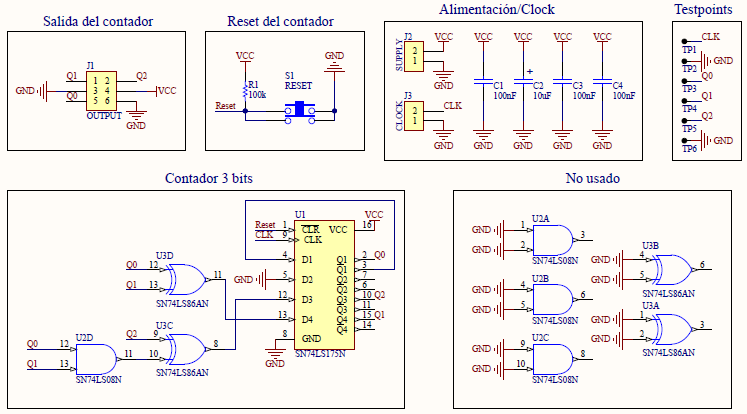
\includegraphics[scale=0.7]{../EJ7/Recursos/esquematico_sincronico.PNG}
    \caption{Esquem\'atico del PCB en Altium Designer}
    \label{fig:esquematico_sincronico}
\end{figure}

\begin{figure}[H]
    \centering
    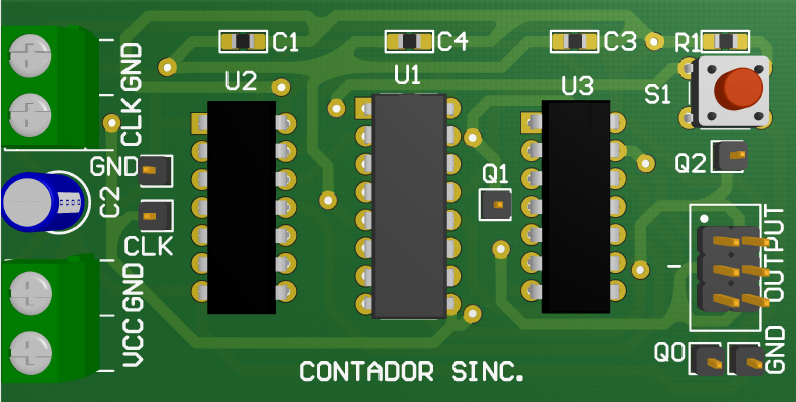
\includegraphics[scale=0.45]{../EJ7/Recursos/3d_top_sincronico.PNG}
    \caption{Dise\~no 3D del PCB}
    \label{fig:3d_sincronico_top}
\end{figure}

\begin{figure}[H]
    \centering
    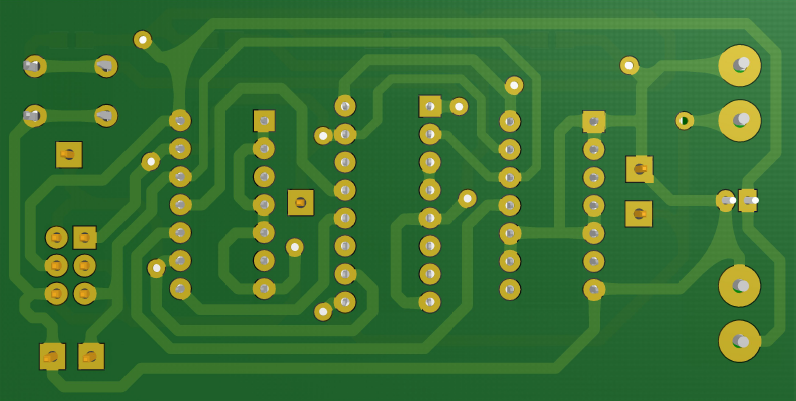
\includegraphics[scale=0.45]{../EJ7/Recursos/3d_bottom_sincronico.PNG} 
    \caption{Dise\~no 3D del PCB}
    \label{fig:3d_sincronico_bottom}
\end{figure}

\subsection{Visualizaci\'on del contador}
Se propone dise\~nar un circuito que decodifique el c\'odigo binario del contador y lo represente en un display
de 7 segmentos para poder realizar una prueba r\'apida del funcionamiento del circuito y poder visualizar el resultado del mismo.

\subsubsection{Dise\~no del circuito}
Se utilizar\'a un circuito integrado 74LS47, esto es, un decodificador BCD a 7 Segmentos, puesto que como la salida del contador se encuentra acotada
entonces puede ser interpretada como BCD. En este integrado la l\'ogica se encuentra negada, por lo cual es necesario utilizar un display de 7 segmentos de \'anodo com\'un,
donde el m\'aximo de corriente que puede soportar la salida del conversor es $25mA$, no obstante se har\'a circular una corriente de $4mA$ por segmento teniendo en cuenta que el modelo utilizado tiene una
tensi\'on $V_{D_ON} \approx 2.7V$.

Asumiendo el peor caso donde la tensi\'on sobre la resistencia es m\'axima y puede circular el m\'aximo de corriente, se limita al valor consignado y por ello se utilizan resistencias
de $R = \frac{5V - 2.7V}{4mA} > 575 \Omega \Rightarrow R = 680 \Omega$.

\begin{figure}[H]
    \centering
        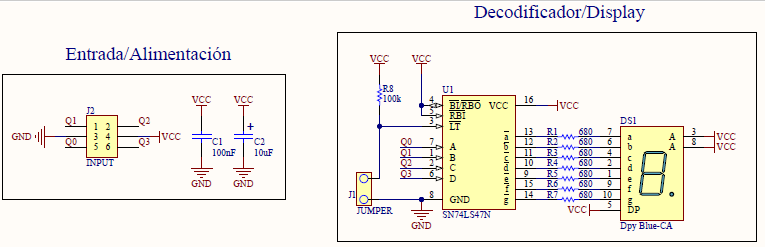
\includegraphics[scale=0.7]{../EJ7/Recursos/esquematico_visualizacion.PNG}
    \caption{Esquem\'atico del PCB en Altium Designer}
    \label{fig:esquematico_visualizacion}
\end{figure}

\begin{figure}[H]
    \centering
    \begin{tabular}{c c}
        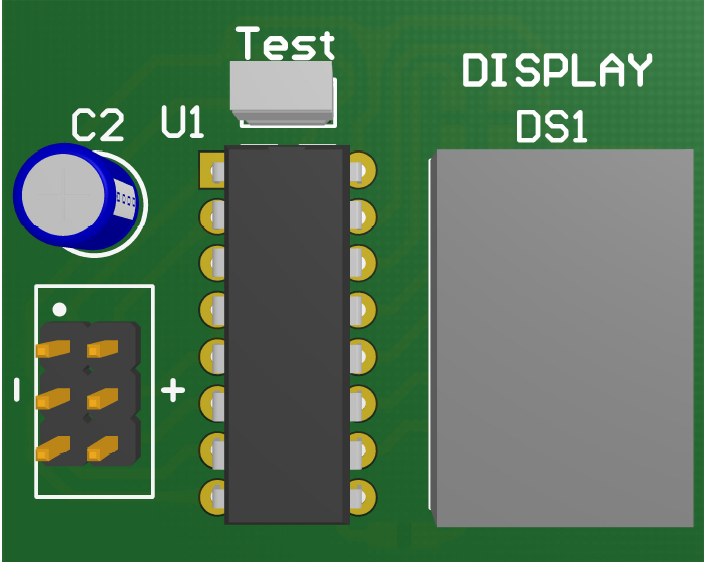
\includegraphics[scale=0.3]{../EJ7/Recursos/3d_top_visualizacion.PNG} &
        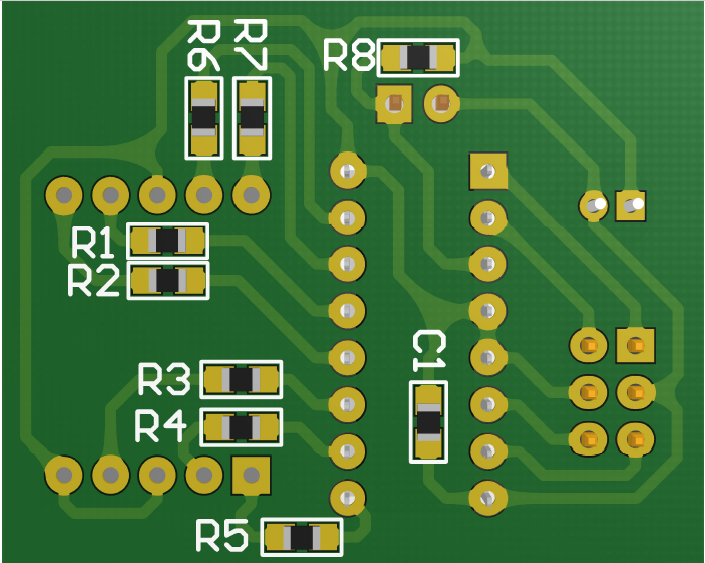
\includegraphics[scale=0.3]{../EJ7/Recursos/3d_bottom_visualizacion.PNG} 
    \end{tabular}
    \caption{Dise\~no 3D del PCB}
    \label{fig:3d_visualizacion}
\end{figure}

\subsection{Resultados}

\begin{figure}[H]
    \centering
        \begin{tabular}{c c}
            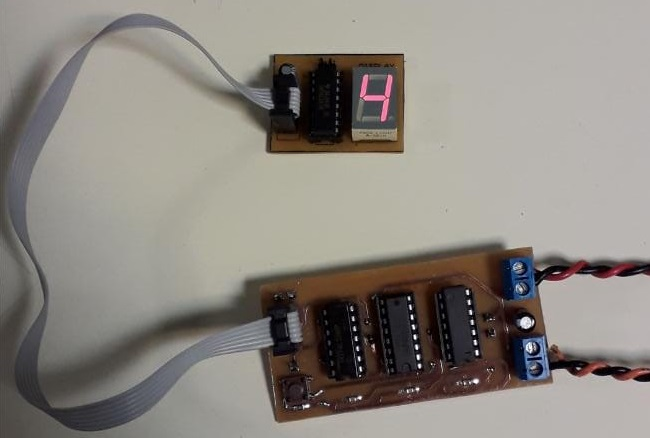
\includegraphics[scale=0.3]{../EJ7/Recursos/practica_0.jpeg} &
            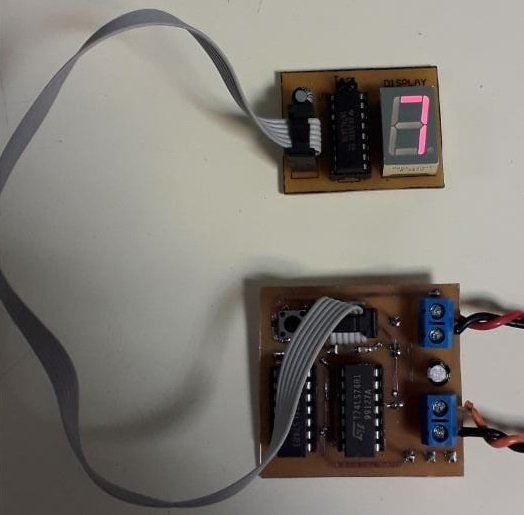
\includegraphics[scale=0.3]{../EJ7/Recursos/practica_1.jpeg}
        \end{tabular}
    \caption{Implementaci\'on de ambos contadores, sincr\'onico y asincr\'onico}
    \label{fig:implementacion}
\end{figure}

\subsubsection{Mediciones}
Para ambos contadores, sincr\'onico y asincr\'onico, se mide por un lado la secuencia del mismo, utilizando los cuatro canales del osciloscopio
para poder observar en color amarillo la se\~nal de clock, la rosa corresponde al $Q_0$, la azul/violeta al $Q_1$ y luego la verde al $Q_2$. Por otro lado,
se mide el tiempo de propagaci\'on de los cambios de cada uno de los flip flops respecto del flanco del clock, para esta \'ultima medici\'on la referencia de colores se mantiene.

\begin{figure}[H]
    \centering
        \begin{tabular}{c c}
            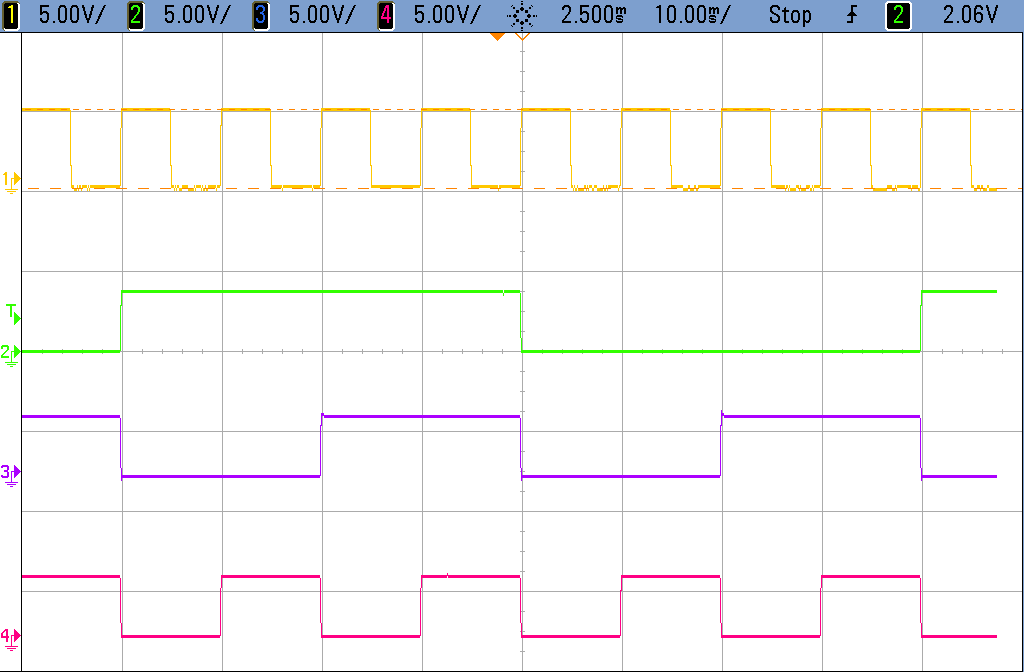
\includegraphics[scale=0.2]{../EJ7/Mediciones/Osciloscopio/Segundo_Intento/Asincronico/cropped_contador.png} &
            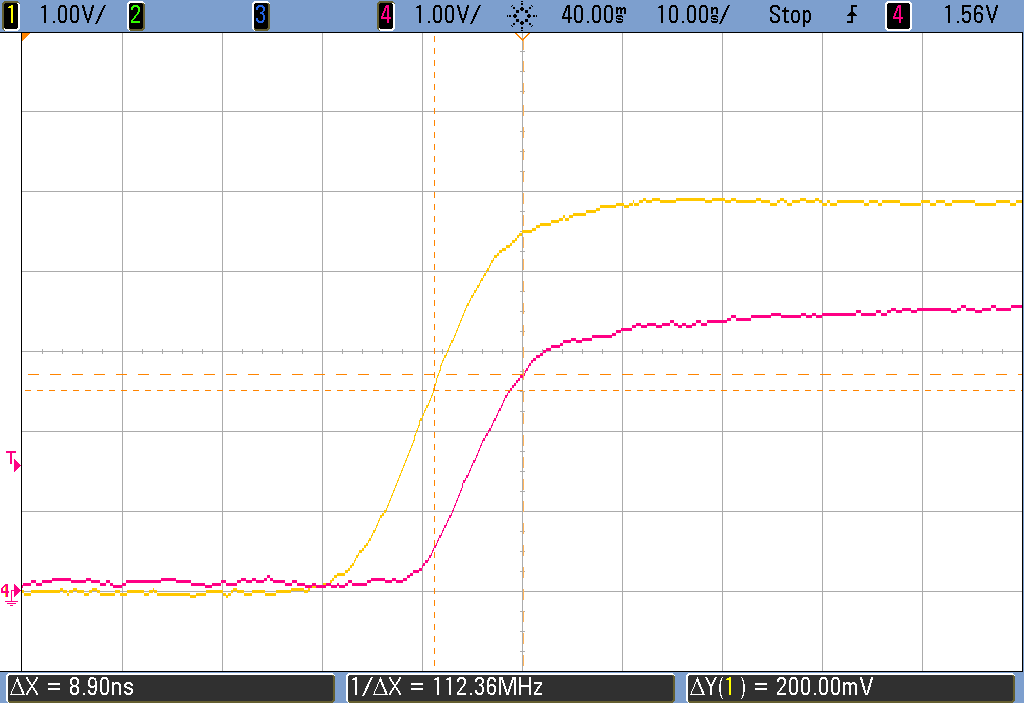
\includegraphics[scale=0.2]{../EJ7/Mediciones/Osciloscopio/Segundo_Intento/Asincronico/cropped_salida_q0.png} \\
            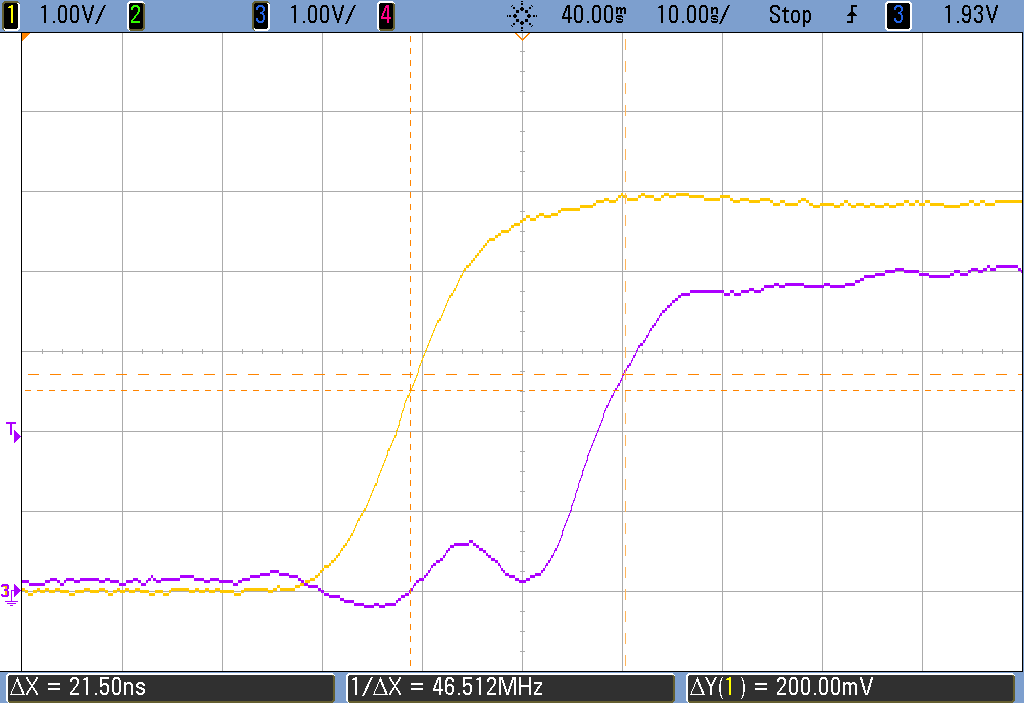
\includegraphics[scale=0.2]{../EJ7/Mediciones/Osciloscopio/Segundo_Intento/Asincronico/cropped_salida_q1.png} &
            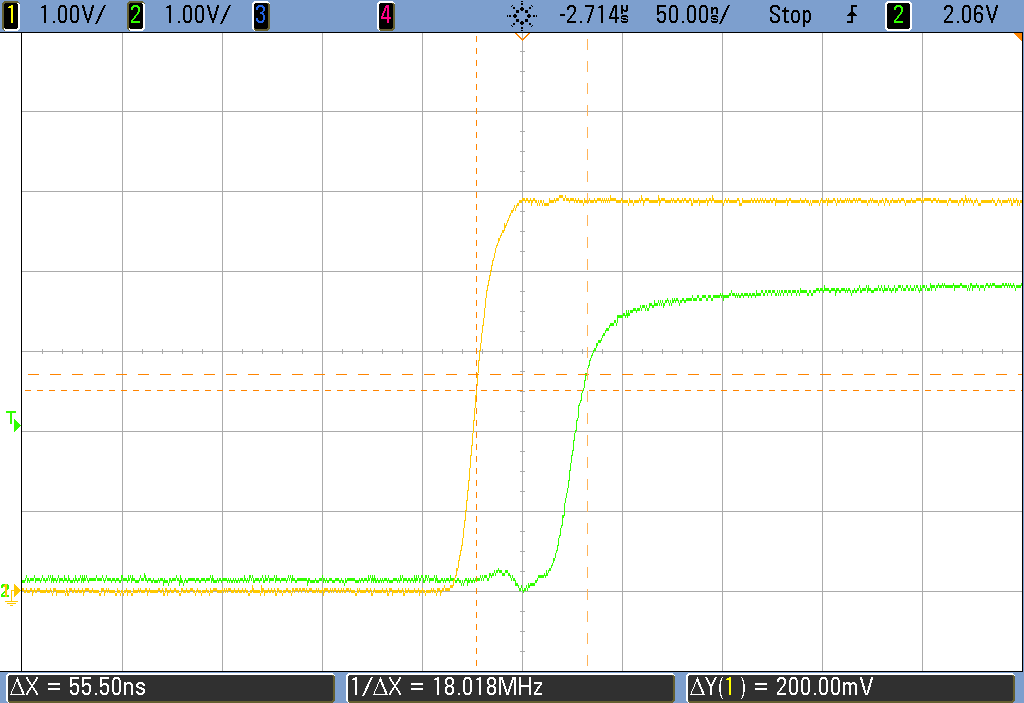
\includegraphics[scale=0.2]{../EJ7/Mediciones/Osciloscopio/Segundo_Intento/Asincronico/cropped_salida_q2.png}
        \end{tabular}
    \caption{Mediciones para Asincr\'onico entre punto medio y $V_{OH}$}
    \label{fig:asincronico_mediciones}
\end{figure}

\begin{figure}[H]
    \centering
        \begin{tabular}{c c}
            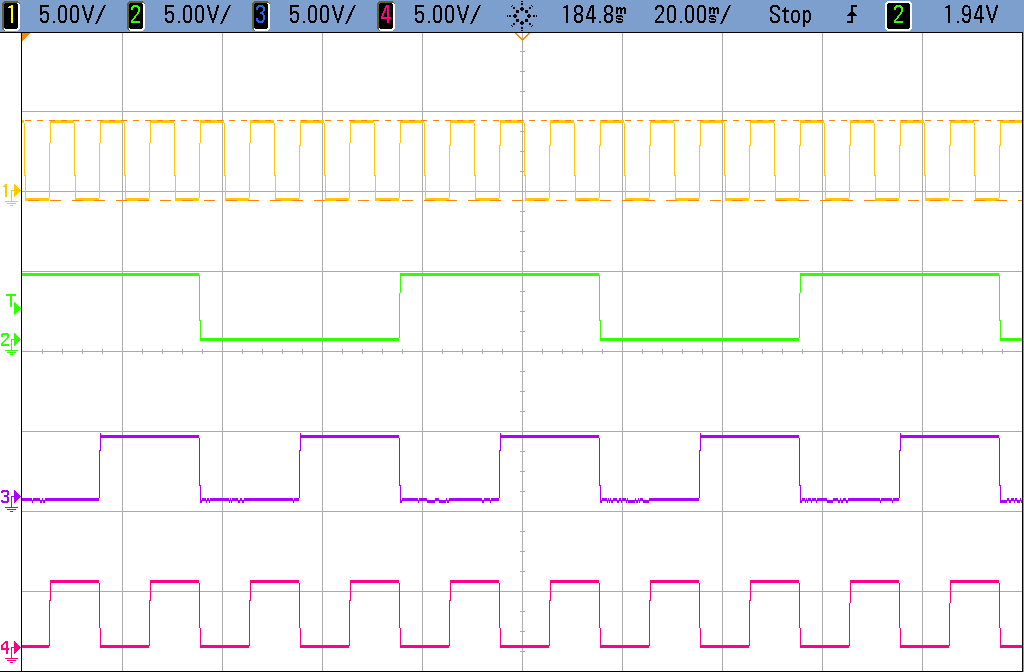
\includegraphics[scale=0.2]{../EJ7/Mediciones/Osciloscopio/Segundo_Intento/Sincronico/cropped_contador.png} &
            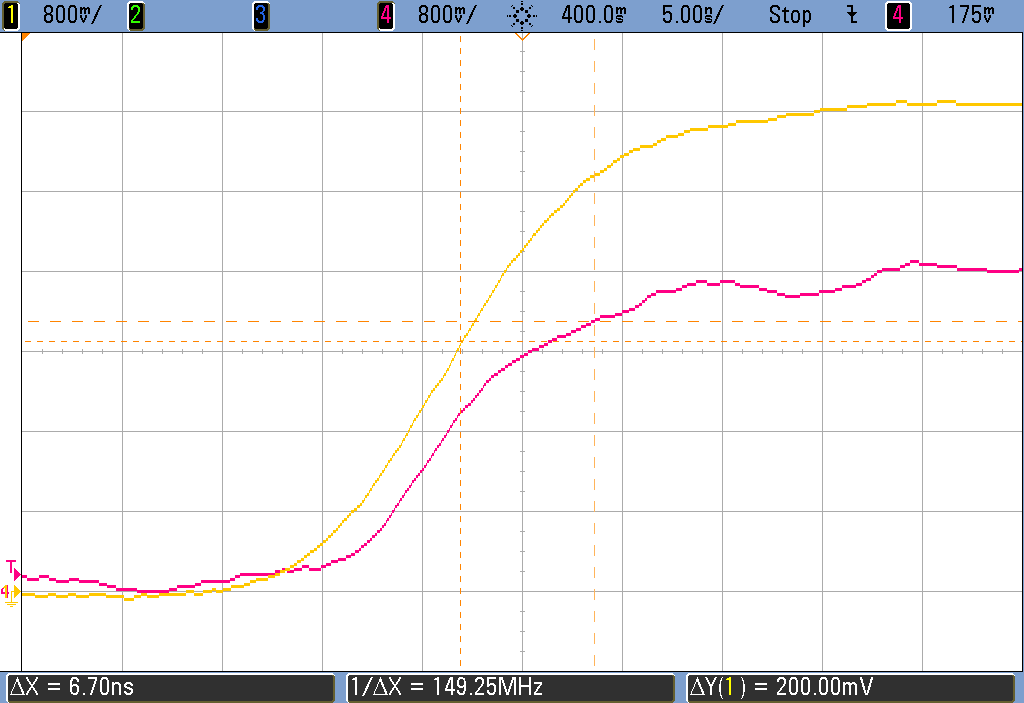
\includegraphics[scale=0.2]{../EJ7/Mediciones/Osciloscopio/Segundo_Intento/Sincronico/cropped_salida_q0.png} \\
            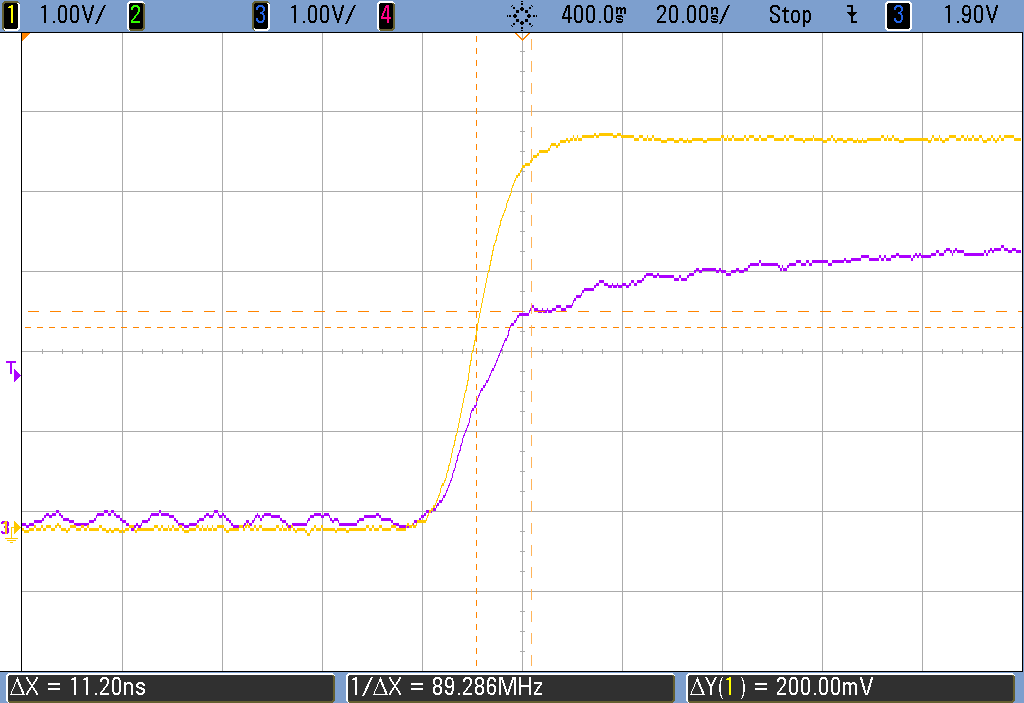
\includegraphics[scale=0.2]{../EJ7/Mediciones/Osciloscopio/Segundo_Intento/Sincronico/cropped_salida_q1.png} &
            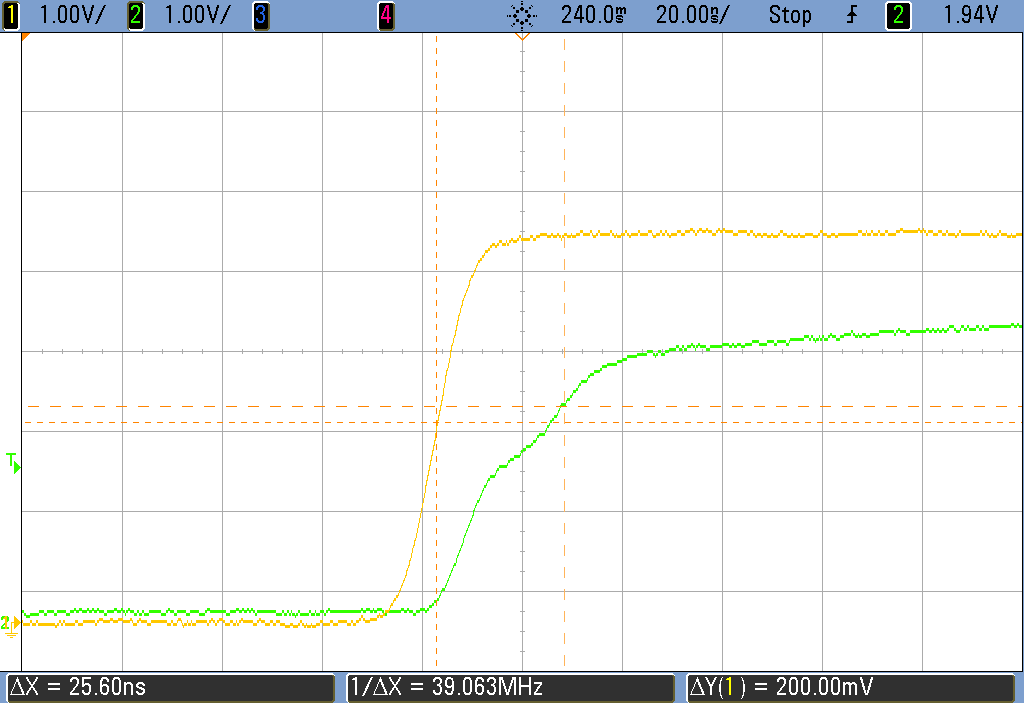
\includegraphics[scale=0.2]{../EJ7/Mediciones/Osciloscopio/Segundo_Intento/Sincronico/cropped_salida_q2.png}
        \end{tabular}
    \caption{Mediciones para Sincr\'onico entre punto medio y $V_{OH}$}
    \label{fig:sincronico_mediciones}
\end{figure}

\subsubsection{An\'alisis de datos}
Resulta de inter\'es observar como anomal\'ia el hecho de que la salida de todos los flip flops no era de $5 V$ sino de $4 V$,
no obstante se encontraba dentro del margen de $V_{OH}$ seg\'un lo provisto por el fabricante. 

En la Fig. \ref{fig:asincronico_mediciones} se puede observar como la forma en que el clock de cada bit depende del anterior en peso produce una propagaci\'on de los tiempos, con lo cual ello explica
la raz\'on de que en esa medida los tiempos hayan ido incrementando bit a bit en el contador. Es por esto que el tiempo de propagaci\'on total
del contador es de $t_p = 55.5nS$, con lo cual cualquier frecuencia de clock que quiera producir un cambio en menos tiempo de esto va a ser ignorada, por ende, limita la frecuencia de operaci\'on a
$f_{MAX} = 18.01MHz$.

En el caso de las mediciones de la Fig. \ref{fig:sincronico_mediciones}, para determinar la frecuencia
m\'axima de operaci\'on es necesario tener en cuenta la respuesta m\'as lenta, es decir, $t_p = 25.6nS \Rightarrow f_{MAX} = 39.03MHz$.

\begin{table}[H]
    \centering
    \begin{tabular}{c c}
        \hline \\
        Contador Asincr\'onico & $f_{MAX} = 18.01MHz$ \\
        Contador Sincr\'onico & $f_{MAX} = 39.03MHz$ \\
        \hline
    \end{tabular}
\end{table}

\subsection{Conclusi\'on}
En conclusi\'on, los procesos sincr\'onicos ser\'an siempre o en la mayor\'ia de los casos m\'as r\'paidos que los proceso asincr\'onicos,
desde el punto de vista en el cual, con un enfoque sincr\'onico se garatiza que los mecanisco involucrados en el funcionamiento de dicho proceso
sean ejecutados o puestos en marcha de forma casi simult\'anea. No sucede as\'i en los procesos asincr\'onicos, como en este contador, donde haya 
una dependencia de tales mecanismos que produzca una propagaci\'on de tiempos que se incrementen.